\documentclass[11pt,a4paper]{article}
\usepackage[utf8]{inputenc}
\usepackage[margin=1in]{geometry}
\usepackage{graphicx}
\usepackage{hyperref}
\usepackage{xcolor}

\begin{document}
\noindent\textbf{\Large Tech Nation Visa - Exceptional Promise}\\
\noindent\textbf{Criteria:} NOT SUBMITTED (replaced by Evidence\_11)\\
\noindent\textbf{Applicant:} Odeyemi Olusegun Israel\\
\rule{\textwidth}{0.4pt}

\vspace{0.5cm}
\begin{center}
    \textbf{\huge Evidence 8: Flutter Consumer App \& Web3 Integration}
\end{center}
\vspace{0.5cm}

\section*{1. Cross-Platform Consumer Application}
Alongside the enterprise compliance dashboard, I engineered an end-user facing application using \textbf{Flutter (Dart)}, targeting all six platforms (iOS, Android, Web, macOS, Windows, Linux) from a single codebase. This mobile-first app acts as the consumer gateway for initiating and approving blockchain transactions that are silently routed through the AMTTP compliance engine.

The Flutter app uses \textbf{Riverpod} for state management, \textbf{go\_router} for navigation, and raw \textbf{dart:js\_util} interop for direct Web3 wallet connectivity --- proving advanced cross-platform engineering that bridges native mobile frameworks with decentralised blockchain protocols.

\vspace{0.3cm}
\noindent\textbf{Flutter App Architecture:}
\begin{itemize}
    \item \textbf{Framework:} Flutter (Dart) --- single codebase targeting iOS, Android, Web, macOS, Windows, Linux
    \item \textbf{State Management:} Riverpod exclusively (ConsumerWidget pattern)
    \item \textbf{Navigation:} go\_router with role-based route guards (R1--R2)
    \item \textbf{Web3 Integration:} Raw \texttt{dart:js\_util} interop for MetaMask/WalletConnect
    \item \textbf{Key Screens:} Home, Wallet Connect, Send Transaction, Transaction History, Trust Check, Disputes
\end{itemize}
\vspace{0.3cm}
\begin{center}
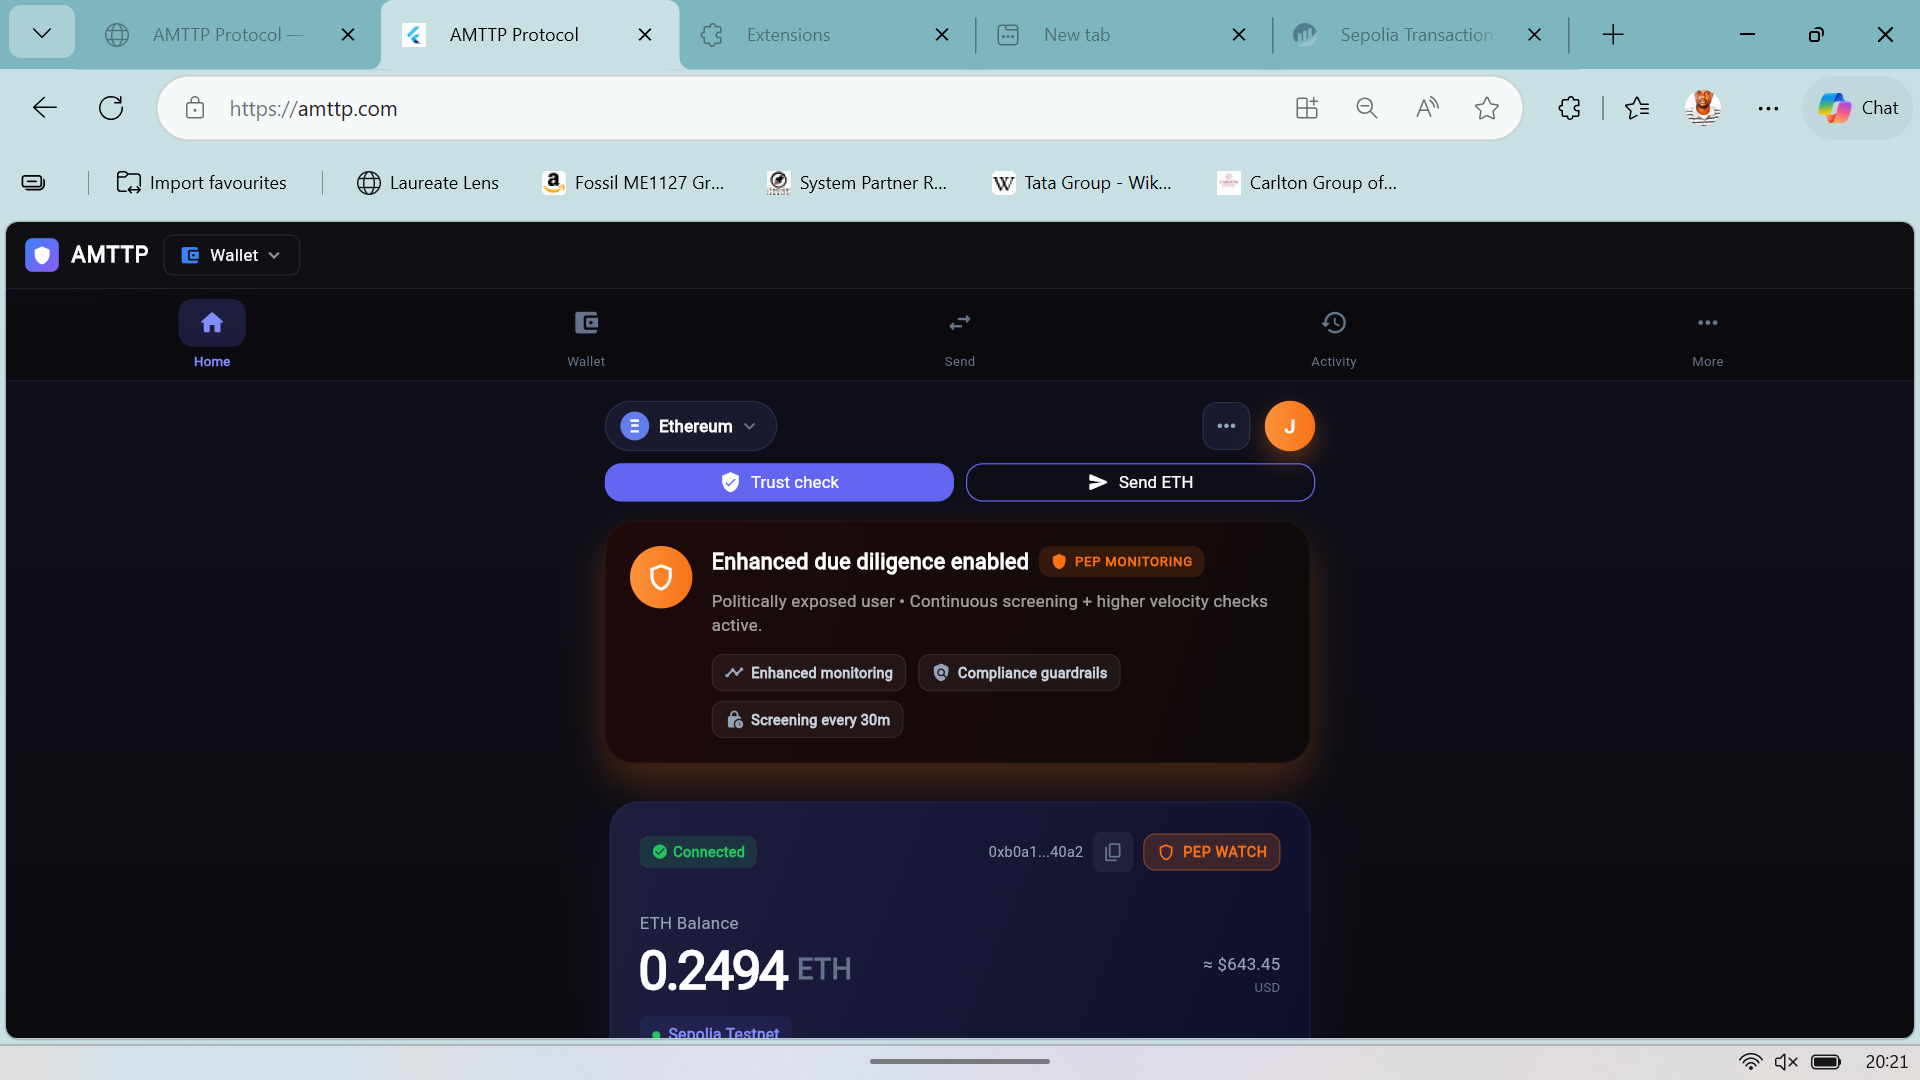
\includegraphics[width=0.85\textwidth]{images/flutter_home_pep.png}
\end{center}
\vspace{0.1cm}
\textit{Figure 1: Live AMTTP consumer app at \texttt{amttp.com} --- MetaMask wallet connected (0.2494 ETH on Sepolia), PEP Monitoring badge with Enhanced Due Diligence enabled, Trust Check and Send ETH actions. Real blockchain integration via raw \texttt{dart:js\_util} interop.}

\section*{2. Smart Contract Verification (On-Chain Finality)}
Every consumer transaction passes through Solidity smart contracts deployed via \textbf{Hardhat (ethers.js v6)} using the \textbf{UUPS upgradeable proxy pattern (OpenZeppelin)}. The contracts enforce an \texttt{onlyOracle} access modifier, ensuring that only the trusted TypeScript Oracle Gateway can submit ML-validated risk scores to the blockchain.

\vspace{0.3cm}
\noindent\textbf{ZK-SNARK On-Chain Verification} (from \texttt{contracts/zknaf/sanctions\_non\_membership\_verifier.sol}):

\vspace{0.2cm}
\noindent\fbox{\begin{minipage}{0.95\textwidth}
\small
\texttt{// Groth16 proof verification --- Sanctions Non-Membership}\\
\texttt{function verifyProof(}\\
\texttt{~~~~uint[2] calldata \_pA,~~~~// Proof element A (G1 point)}\\
\texttt{~~~~uint[2][2] calldata \_pB, // Proof element B (G2 point)}\\
\texttt{~~~~uint[2] calldata \_pC,~~~~// Proof element C (G1 point)}\\
\texttt{~~~~uint[4] calldata \_pubSignals // Public inputs}\\
\texttt{) public view returns (bool) \{}\\
\texttt{~~~~assembly \{}\\
\texttt{~~~~~~~~// BN254 G1 scalar multiplication via precompile 7}\\
\texttt{~~~~~~~~g1\_mulAccC(\_pVk, IC1x, IC1y, calldataload(pubSignals))}\\
\texttt{~~~~~~~~g1\_mulAccC(\_pVk, IC2x, IC2y, calldataload(add(pubSignals, 32)))}\\
\texttt{~~~~~~~~// Pairing check via precompile 8: e(A,B)*e(vk\_x,gamma)*e(C,delta)=1}\\
\texttt{~~~~~~~~isOk := and(success, mload(\_pPairing))}\\
\texttt{~~~~\}}\\
\texttt{\}}
\end{minipage}}
\vspace{0.2cm}

\noindent\textit{Figure 2: Groth16 ZK-SNARK proof verification in Solidity --- proves sanctions non-membership on-chain using BN254 elliptic curve pairings, without revealing the user's identity or transaction metadata.}

\vspace{0.3cm}
\begin{center}
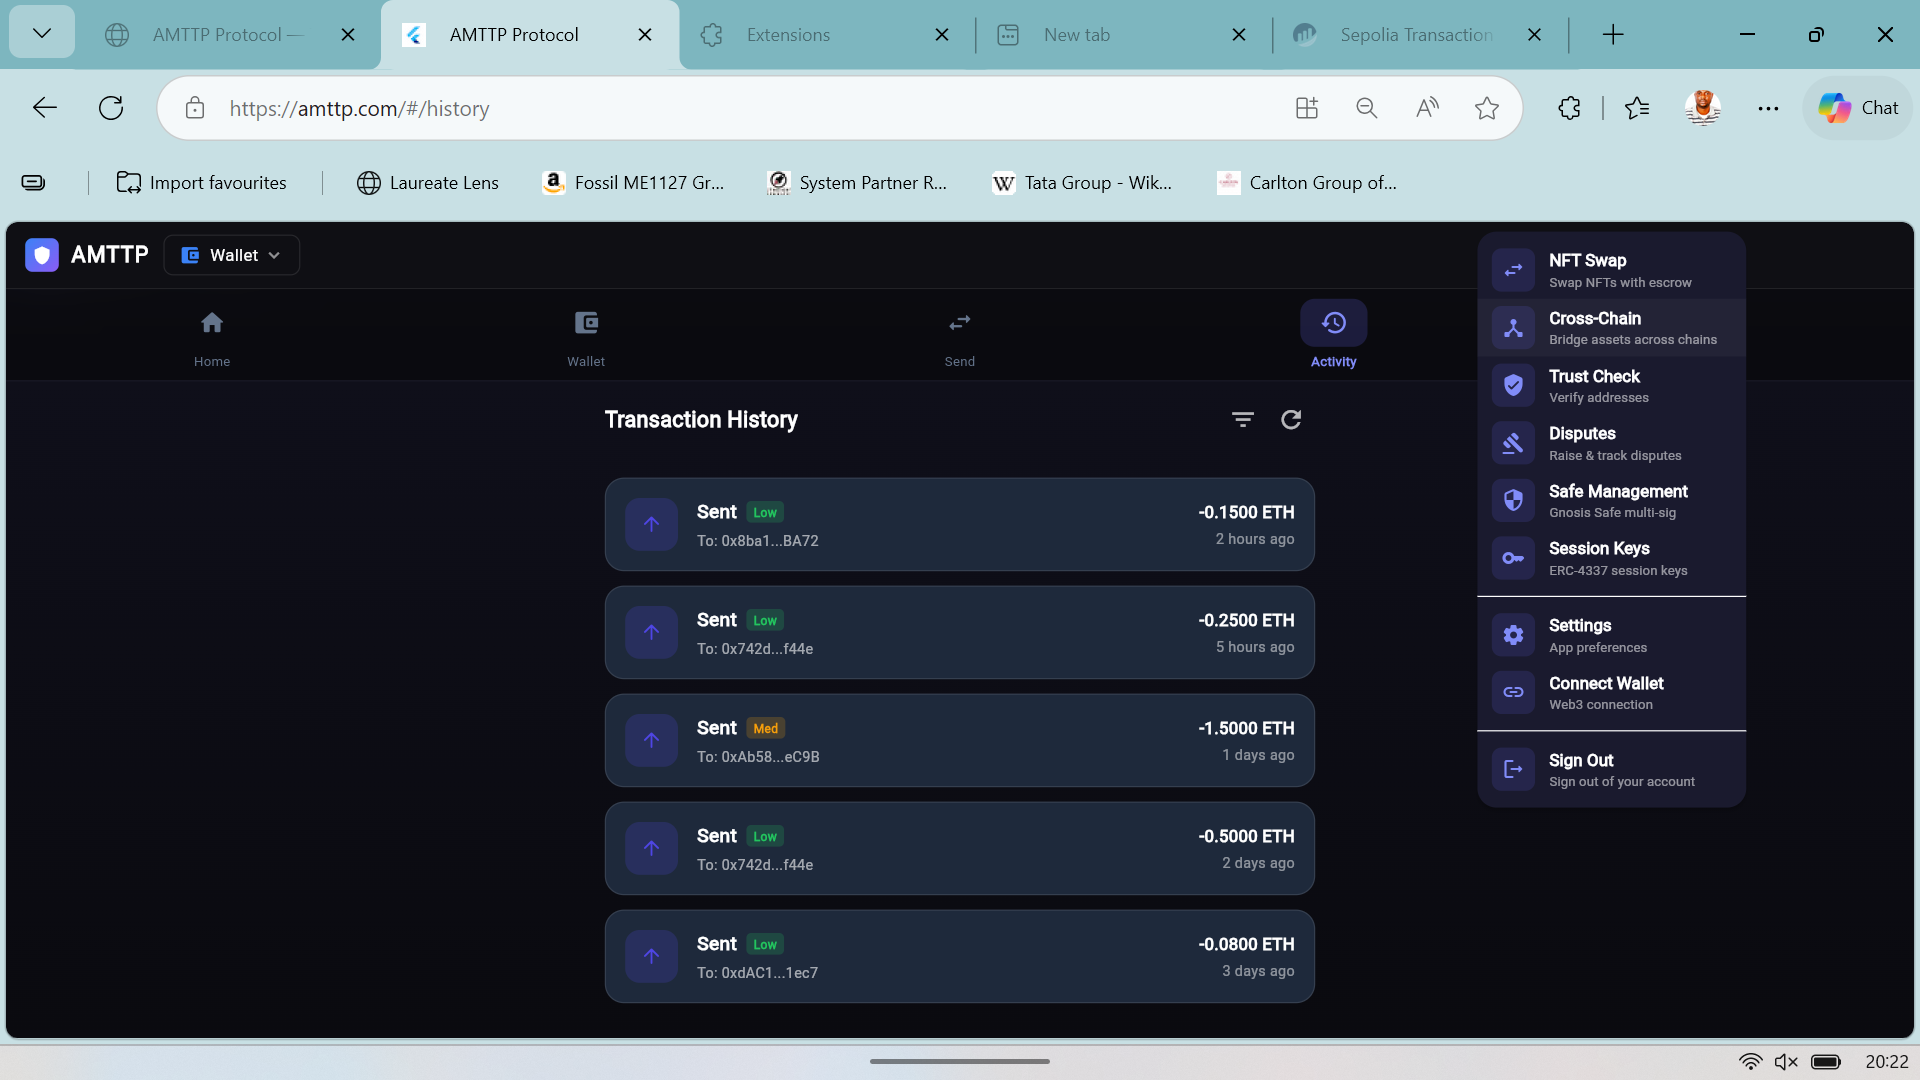
\includegraphics[width=0.85\textwidth]{images/flutter_activity_menu.png}
\end{center}
\vspace{0.1cm}
\textit{Figure 3: Transaction History with risk-level badges (Low/Med) and expanded navigation showing all consumer features --- NFT Swap, Cross-Chain bridging, Trust Check, Disputes, Safe Management (Gnosis multi-sig), and ERC-4337 Session Keys.}

\section*{3. End-to-End Proof of Concept}
The complete flow --- from mobile app transaction request, through off-chain ML risk scoring, to on-chain ZK-proof validation and settlement --- represents a differentiated architectural contribution to the Web3 compliance space. To the best of my knowledge, very few open-source or commercial products integrate all of these layers within a single independently built system.

\end{document}